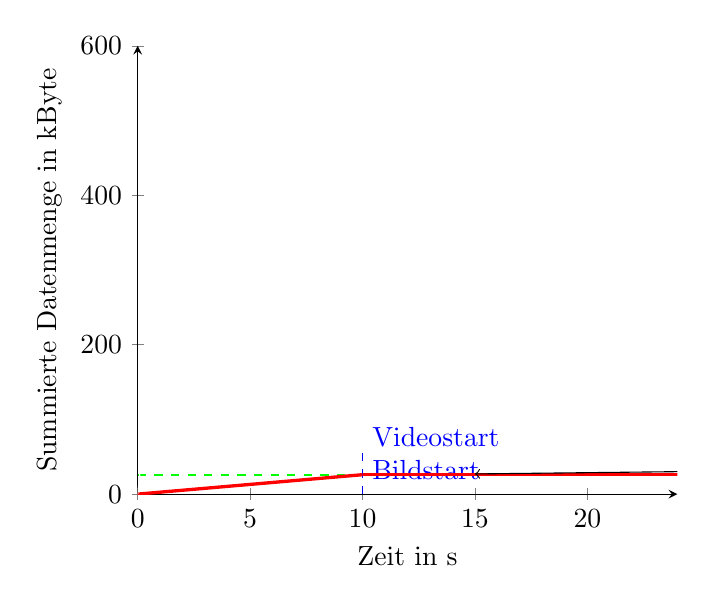
\begin{tikzpicture}
	\begin{axis} [domain=0:24, xlabel={Zeit in s}, ylabel={Summierte Datenmenge in $ \mathrm{kByte} $}, axis x line=bottom, axis y line=left, ymin=0, ymax=600, xmin=0, xmax=24]
		\draw[blue, dashed] (10, 0) -- (10, 60);
		\node[blue, right, dotted, text width=2cm] at (10, 55) (S1) {Videostart Bildstart};
		\draw[blue, dashed] (110, 0) -- (110, 60);
		\node[blue, right, dotted] at (110, 57) (S2) {Videoende};
		\draw[blue, dashed] (100, 40) -- (100, 60);
		\draw[->] (110, 40) -- node[below] {$ 1\,\mathrm{s} $}(100,400);
		\draw[green, dashed, thick] (0, 26) -- (240, 26);	
		\node[above, green] at (150, 26) {Datenmenge bei Videostart};
		\draw[red, very thick] (0,0) -- (10, 26);
		\draw[red, very thick] (10, 26) -- node[below, text width=3cm] {Minimum Datenübertragung} (100, 26);
		\addplot[white] expression {564.2/190 * x * 100};
		\node[right]  (K1) at (30, 34) {1. kritischer Punkt};
		\draw[->] (K1) -- (15, 27);
	\end{axis}
\end{tikzpicture}